\chapter{Introduction}\label{ch:introduction}

This report is submitted as part of the assessment for the authors enrolment in Masters class The Art of Scientific 
Computation at the University of Melbourne. The report outlines the process the author went through when 
completing the Respiratory Rate research project. 

\section{Motivation and Biological Background}
Respiratory rate, defined as the number of complete breaths per minute, is a fundamental 
vital sign, with importance across healthcare and exercise science \cite{ala2025respiratory_rate},\cite{nicolo2020importance}. 
A persons Respiratory Rate is impacted by a number of factors including injury, illness or stress, adding difficulty 
to the measurement process, however 
it is an extremely important vital as abnormal Respiratory Rate is often the first indicator 
of illness \cite{ala2025respiratory_rate}. Despite this, Respiratory Rate monitoring is still 
not performed routinely in the healthcare setting, which may be due to the lack of standard 
Respiratory Monitoring technology \cite{nicolo2020importance}. One area of critical importance 
in Respiratory Rate Estimation is finding a low-cost, consistent and robust method for measuring 
Respiratory Rate, this is most critical in rural, low income areas where the lack of accurate, easy 
to obtain measurements may led to patients being incorrectly sent home \cite{valerian2026respiratory}, \cite{nicolo2020importance}.
This issue is pertintent to diagnosis of Pneumonia, especially in children; Pneumonia is responsible for 14\% of all deaths of children 
under 5, despite pneumonia being  easily treatable with widely available oral medication, indicating the importance of being able to 
effectively diagnose in settings where resources are scarce \cite{who2022pneumonia}. Respiratory Rate can be an indicator of severe pneumonia, 
and the World Health Organisation suggest that Respiratory Rate is integral to the diagnosis pathway;
further illustrating the criticality of determining reliable methods for measurement. \cite{nicolo2020importance}.\\


An area of active research is developing a method for reliably estimating  Respiratory Rate via electrocardiogram (ECG) signals.
ECGs are a non-invasive, widely available tool used in healthcare that measures the electrical activity of the heart, specifically 
volatage over time. Electrodes (typically 10) are placed on a person lying down, these electrodes measure the magnitude
of the electric potential from 12 different angles - this is called a 12 lead ECG \cite{wikipedia_electrocardiography}. 
 A normal ECG signal is made up of 3 parts, the P-wave, QRS complex and T wave associated to 
 different activities of the hearts beating cycle \cite{wikipedia_electrocardiography}. Figure~\ref{fig:sinus} illustrates 
the characteristics of each part. 
\begin{figure}[H]
    \centering
    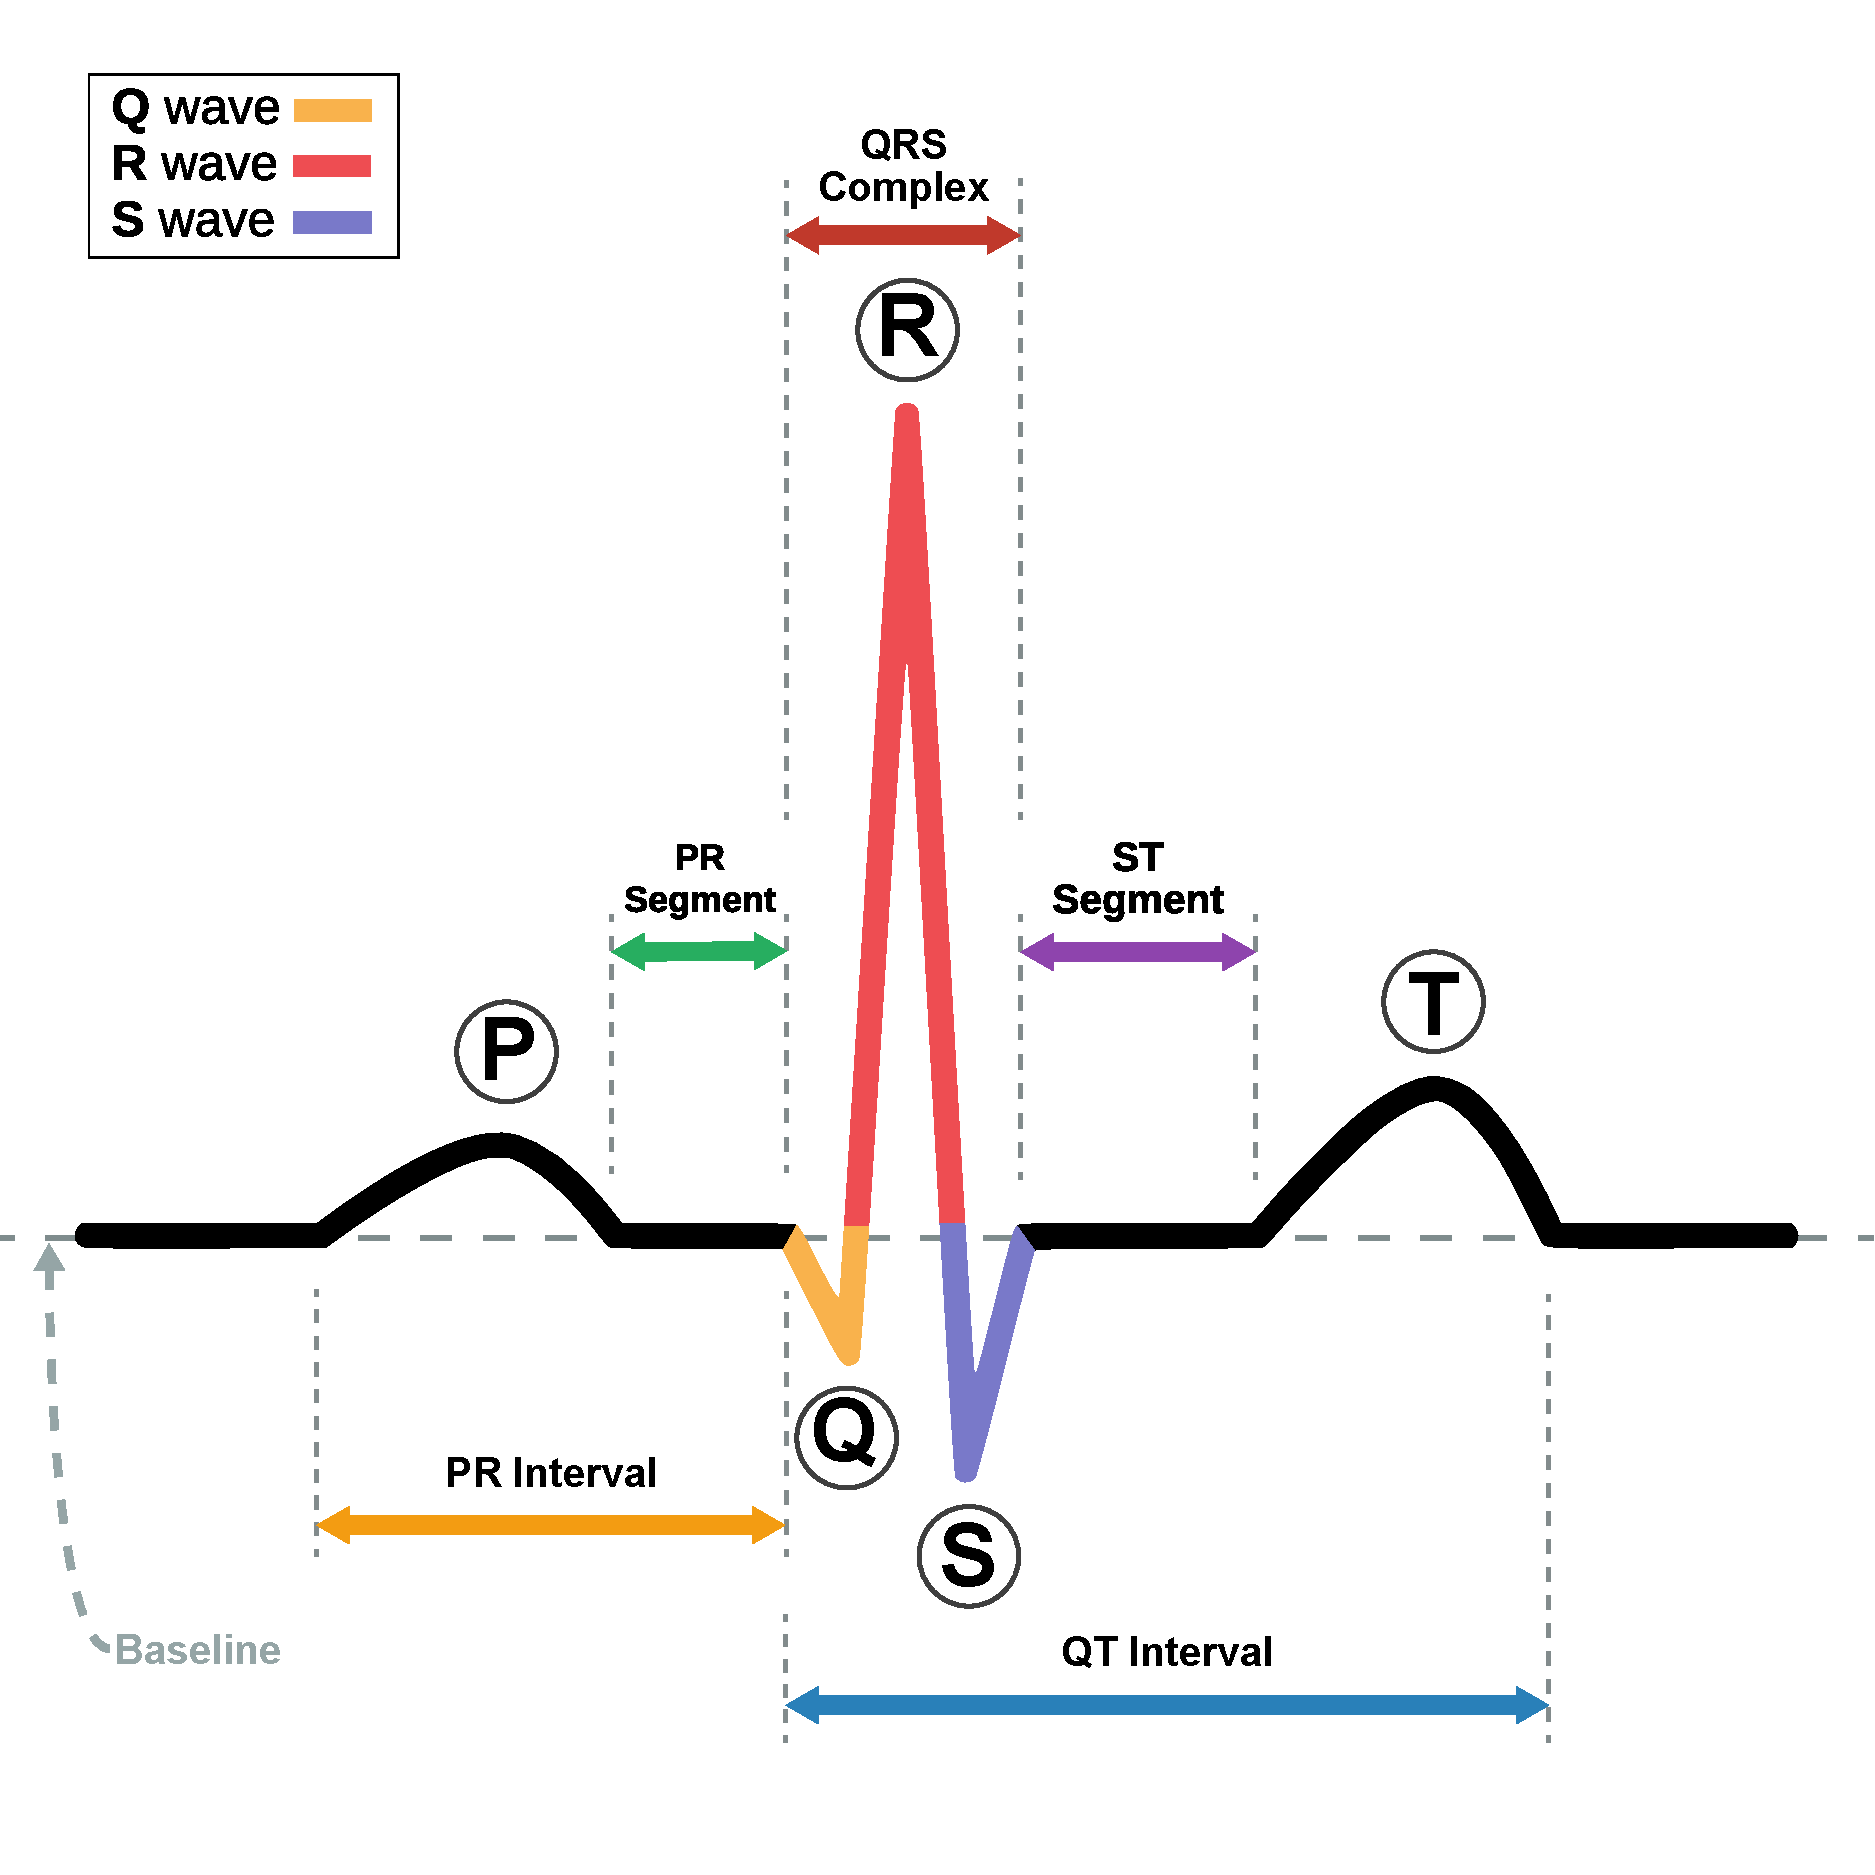
\includegraphics[width=0.50\textwidth]{figures/SinusRhythmLabels.pdf}
    \caption{Notated diagram of a Sinus Rhythm, the signal generated by an ECG \cite{wikipedia_electrocardiography}.}
    \label{fig:sinus}
\end{figure}
Of interest to this project is the QRS complex characterised by large short peaks on the ECG signal, it corresponds to repolarisation of the 
ventricles, that is the contraction of the heart to pump out blood \cite{wikipedia_electrocardiography}. There are two commonly used methods 
that use waveforms create by these peaks (sometimes refered to as RR peaks), to estimate Respiratory Rate providing a potential 
low-cost widely available methods for measuring Respiratory Rate. The first challenge will thus be, being able to robustly
identify the location of QRS complexes in an ECG signal, which poses a challenge due to the sensitivity of ECG signals 
to noise and artifacts. 

\newpage

\section{Research Methodology}
The predominant Goal of this project is two fold, firstly we develop a method for identifying 
QRS complexes on an ECG signal, from which we use this algorithm to evalute methods for estimating Respiratory Rate from 
different waveforms that stem from patterns in the QRS complexes occurence and amplitude.
The methods we will evaluate analyse characteristics of the waveform namely how the 
time between QRS complexs varies - refered to as the RSA method or how the amplitude 
of the waveform varies - refered to as the RPA method. We will employ spectrum associated methods (Fast Fourier Transform or Lomb-Scargle) 
to try an identify a dominate, roughly consistent frequency in the expected Respiratory Rate range that 
will become the estimated Respiratory Rate. \\
Our Methodology will go as follows:
\begin{enumerate}
        \item Investigate ECG signals, identifying datasets with distinct varying behaviour to test the Robustness of our algorithms.
        This is described in Section 2.
        \item Develop, evaluate and refine an algorithm to robustly identify RR peaks, testing the performance 
        against annotations for the occurence of a QRS complex. This is described in Section 3.
        \item Evaluate and test different methods for estimating Respiratory Rate, by analysing their ability 
        to detect a strong, consistent frequency that with high probability is the Respiratory Rate. This is described in Section 4.
\end{enumerate}